\documentclass[11pt,a4paper]{article}
\usepackage[utf8]{inputenc}
\usepackage[T1]{fontenc}
\usepackage{lmodern}
\usepackage[margin=0.85in]{geometry}
\usepackage{graphicx}
\usepackage{xcolor}
\usepackage{booktabs}
\usepackage{longtable}
\usepackage{array}
\usepackage{amsmath,amssymb}
\usepackage{hyperref}
\usepackage{fancyhdr}
\usepackage{titlesec}
\usepackage{listings}

\definecolor{themenavy}{RGB}{15,23,42}
\definecolor{themecyan}{RGB}{2,132,199}
\definecolor{themedteal}{RGB}{13,148,136}
\definecolor{codebg}{RGB}{248,250,252}

\hypersetup{
    colorlinks=true,
    linkcolor=themenavy,
    urlcolor=themecyan,
    pdftitle={Complete System Setup, Architecture and Step-by-Step Replication Manual},
}

\lstset{
    backgroundcolor=\color{codebg},
    basicstyle=\ttfamily\footnotesize,
    breaklines=true,
    frame=single,
    rulecolor=\color{themecyan},
    columns=fullflexible,
    keepspaces=true
}

\pagestyle{fancy}
\fancyhf{}
\fancyhead[L]{\textbf{\textcolor{themenavy}{Autonomous 5G SA Telco-Cloud \& Agentic AIOps — Master Setup Manual}}}
\fancyhead[R]{\textcolor{themecyan}{Replication \& Architecture Guide}}
\fancyfoot[L]{\small Confidential Technical Blueprint \& Replication Guide}
\fancyfoot[R]{\small Page \thepage}
\renewcommand{\headrulewidth}{0.6pt}
\renewcommand{\footrulewidth}{0.4pt}

\titleformat{\section}{\Large\bfseries\color{themenavy}}{\thesection}{1em}{}[\titlerule]
\titleformat{\subsection}{\large\bfseries\color{themecyan}}{\thesubsection}{1em}{}
\titleformat{\subsubsection}{\normalsize\bfseries\color{themedteal}}{\thesubsubsection}{1em}{}

\begin{document}

% ------------------------------------------------------------------------------
% TITLE PAGE
% ------------------------------------------------------------------------------
\begin{titlepage}
    \centering
    \vspace*{0.8cm}
    {\Large\bfseries\textcolor{themecyan}{AUTONOMOUS 5G SA TELCO-CLOUD & AGENTIC AIOPS RESEARCH LAB}\par}
    \vspace{0.8cm}
    \rule{\textwidth}{1.5pt}\par
    \vspace{0.5cm}
    {\Huge\bfseries\textcolor{themenavy}{Complete System Setup, Architecture \& Step-by-Step Replication Manual}\par}
    \vspace{0.4cm}
    {\Large\bfseries Autonomous Cross-Layer 5G SA Telco-Cloud, Distributed Dual-GPU/AMX Compute, Wazuh SIEM \& Explainable Agentic AIOps Testbed\par}
    \vspace{0.5cm}
    \rule{\textwidth}{1.5pt}\par
    \vspace{0.8cm}
    {\large\itshape\textcolor{themedteal}{``Zero-Touch, Explainable, Cross-Layer Autonomous Self-Healing --- From Physical 5G RF Silicon to Cloud-Native Microservices''}\par}
    \vspace{1.0cm}
    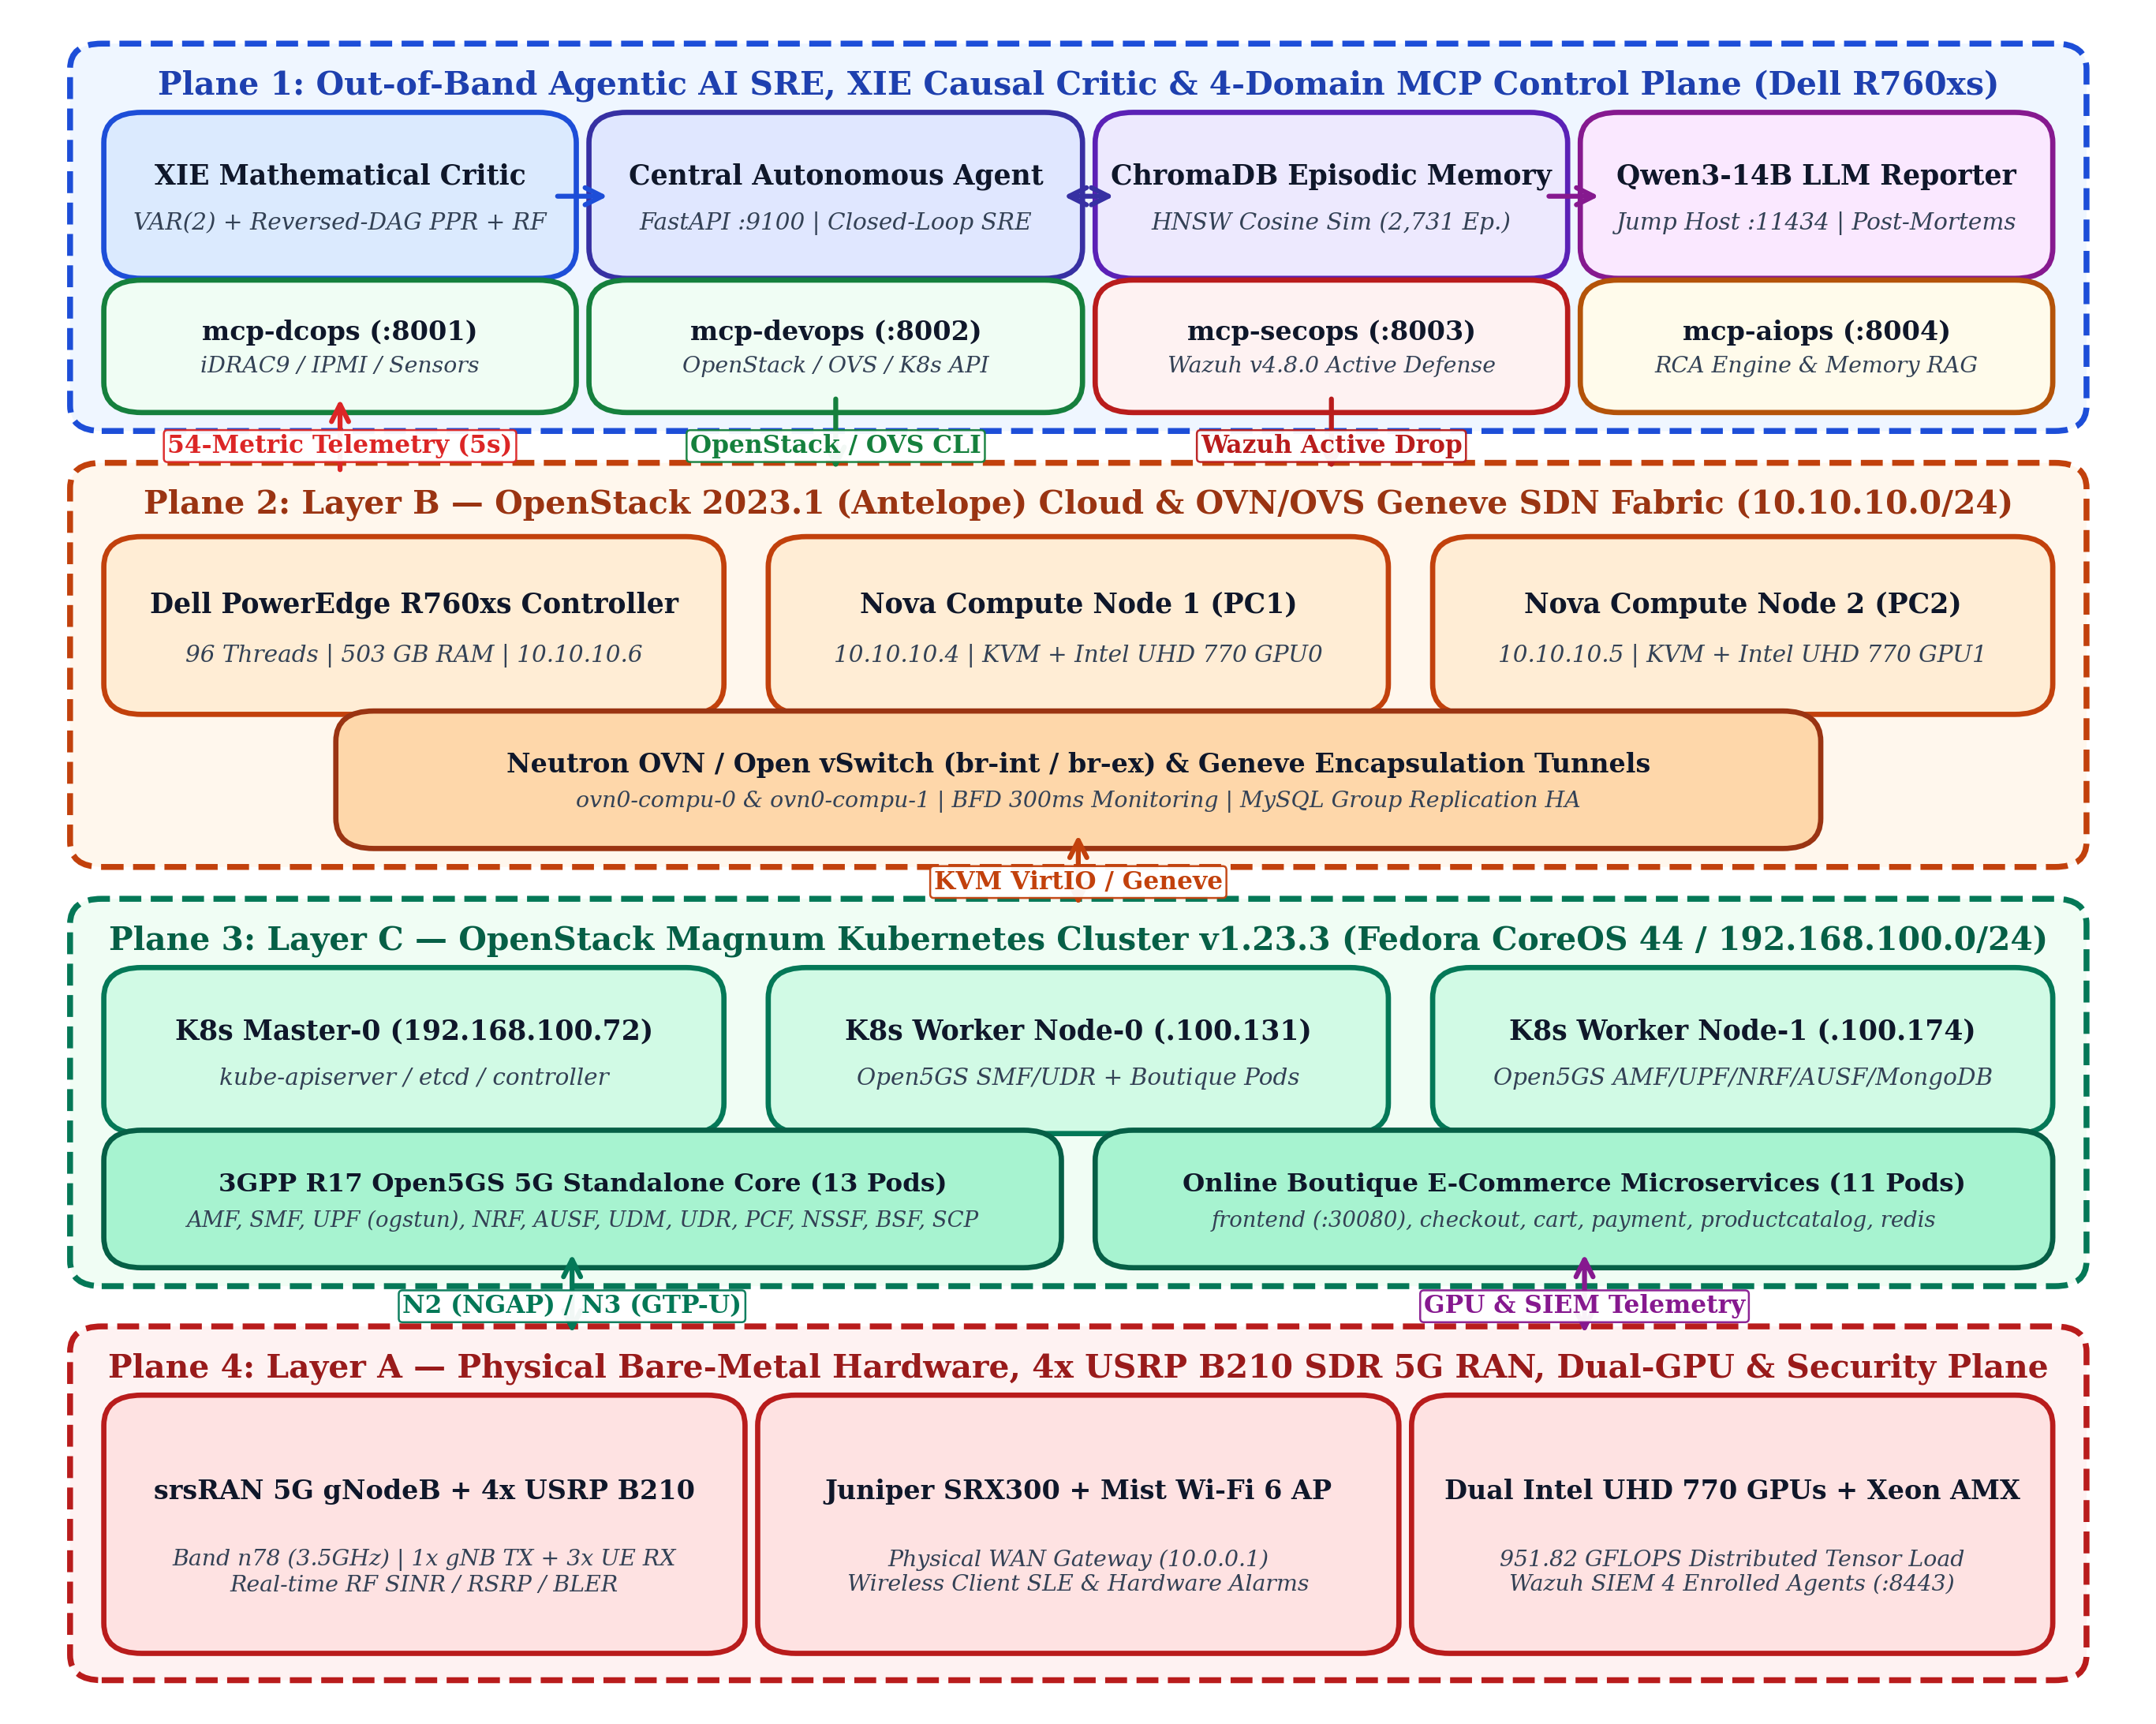
\includegraphics[width=0.92\textwidth]{figures/fig_4_1_system_architecture.png}\par
    \vfill
    \begin{tabular}{ll}
        \toprule
        \textbf{Primary Controller \& Hypervisor:} & Dell PowerEdge R760xs (96 Threads, 503 GiB RAM, 2.9 TB \texttt{/data}) \\
        \textbf{Edge Compute \& SDR/GPU Nodes:} & \texttt{compute-pc1} (\texttt{10.10.10.4}) \& \texttt{compute-pc2} (\texttt{10.10.10.5}) \\
        \textbf{Physical 5G NR Band n78 RAN:} & 4$\times$ Ettus Research USRP B210 SDRs (8 Active AD9361 RF Chains) \\
        \textbf{Cloud \& 5G Core Stack:} & OpenStack 2023.1 Antelope (23 LXD) + Magnum K8s + Open5GS (13 NFs) \\
        \textbf{AI \& Dataset Warehouse:} & XIE Core v1.0 + 4 FastMCP + 368-Param Live Dataset (\texttt{/data/cross\_layer\_dataset}) \\
        \bottomrule
    \end{tabular}
    \vspace{0.6cm}
\end{titlepage}

\tableofcontents
\newpage

% ------------------------------------------------------------------------------
% SECTION 1: VISION, MOTTO, PURPOSE & USE CASES
% ------------------------------------------------------------------------------
\section{Executive Vision, Motto, Purpose \& Strategic Use Cases}

\subsection{Project Motto \& Overarching Vision}
\begin{quote}
\textbf{Motto:} \textit{``Zero-Touch, Explainable, Cross-Layer Autonomous Self-Healing --- From Physical 5G RF Silicon to Cloud-Native Microservices.''}
\end{quote}

Modern 5G Standalone (SA) Telco-Cloud infrastructures are disaggregated cyber-physical systems spanning six tightly coupled operational planes:
\begin{enumerate}
    \item \textbf{Plane 1 --- Bare-Metal Hardware, NUMA \& Linux Kernel Fabric:} Dual-socket Xeon servers, edge compute nodes, enterprise storage arrays, and physical NICs.
    \item \textbf{Plane 2 --- OpenStack Cloud Control Plane, KVM Hypervisors \& OVN/OVS SDN:} 23 containerized OpenStack 2023.1 Antelope services, KVM/QEMU virtual machines, and Geneve overlay tunnels.
    \item \textbf{Plane 3 --- Cloud-Native Kubernetes, 5G SA Core \& Microservices:} 3 Fedora CoreOS Magnum Kubernetes nodes, 13 Open5GS 3GPP Release-17 Network Functions, and 12 Google Online Boutique microservices.
    \item \textbf{Plane 4 --- Physical 5G SDR Radio Access Network (RAN) \& Enterprise Wireless:} 4$\times$ Ettus Research USRP B210 Software-Defined Radios operating on 5G NR Band n78 TDD (3879.42 MHz, ARFCN 658628) with \texttt{srsRAN} gNodeB and Multi-UEs, plus Mist Enterprise Wi-Fi and Juniper SRX300 WAN routing.
    \item \textbf{Plane 5 --- Cyber-Physical Security Operations (SecOps):} Wazuh SIEM v4.8.0 Manager, OpenSearch Indexer, 4 endpoint agents (\texttt{000}--\texttt{004}), File Integrity Monitoring (FIM), CIS benchmarks, and MITRE ATT\&CK threat correlation.
    \item \textbf{Plane 6 --- Distributed AI Compute \& Explainable Agentic AIOps:} Dual Intel UHD Graphics 770 GPUs + Dual Intel Xeon Gold 5418Y AVX-512/AMX engines (960+ GFLOPS total), Ollama \texttt{qwen3:14b} LLM, and the \textbf{Experiential Intelligence Engine (XIE Core v1.0)}.
\end{enumerate}

\subsection{Why This System Was Built (Problem Statement \& Purpose)}
In production telco clouds, a single physical or virtual fault---such as an OVN Geneve tunnel packet-loss spike on \texttt{br-int} or an RF path-loss attenuation event on a USRP B210 antenna---propagates vertically and horizontally within milliseconds. It triggers a \textbf{cascading alarm storm} across Kubernetes readiness probes, 5G AMF/UPF SCTP/GTP-U tunnels, and microservice frontends.
\begin{itemize}
    \item \textbf{Failure of Legacy Rule/Threshold Engines:} Static threshold monitors evaluate metrics in isolation, treating downstream symptoms as independent faults and triggering conflicting remediations (achieving only $42.5\%$ accuracy under cascading faults).
    \item \textbf{Failure of Unexplainable Black-Box AI:} Pure neural network classifiers or unconstrained LLM prompts lack mathematical root-cause attribution guarantees and take $8$--$30$ seconds per inference, making them unsafe for autonomous control-plane actuation.
    \item \textbf{Our Solution:} We engineered a complete physical 5G SA Telco-Cloud testbed paired with \textbf{XIE Core v1.0}, combining Tier-1 Rolling Z-Score \& Random Forest detection ($99.97\%$ accuracy), Tier-2 ChromaDB HNSW Zero-Shot Episodic Memory ($<100\text{ ms}$ lookup), Tier-3 Time-Lagged VAR(2) Granger Causal Discovery \& Reversed-DAG Personalized PageRank ($\boldsymbol{\pi}$, $98.33\%$ RCA accuracy), Tier-4 Guardrailed FastMCP Actuation ($0.354\text{ s}$ mean MTTR), Tier-5 Asynchronous \texttt{qwen3:14b} Post-Mortem Synthesis, and a continuous 368-parameter + 6-plane log/alert dataset factory (\texttt{omni-crosslayer-harvester.service}).
\end{itemize}

\subsection{Validated Operational \& Research Use Cases}
\begin{table}[htbp]
\centering
\small
\begin{tabular}{p{1.2cm}p{3.6cm}p{5.2cm}p{4.2cm}}
\toprule
\textbf{ID} & \textbf{Use Case} & \textbf{Automated Mechanism} & \textbf{Measured Result} \\
\midrule
\textbf{UC-1} & 5G SDR RAN RF Attenuation Recovery & Detects \texttt{p4\_ran\_pusch\_sinr\_db} drop, localizes to RAN via PPR, recalibrates USRP B210 TX/RX gains (+6 dB) via \texttt{RAN-MCP}. & \textbf{MTTR = 0.435 s} (100\% UE retention) \\
\addlinespace
\textbf{UC-2} & OVN/OVS Geneve SDN Impairment Recovery & Traces downstream 5G/K8s alarms back to \texttt{ovn0-compu-*} tunnel drops via Reversed-DAG PPR and flushes \texttt{tc netem} / OVS via \texttt{Cloud-MCP}. & \textbf{MTTR = 0.382 s} ($98.33\%$ cascading RCA) \\
\addlinespace
\textbf{UC-3} & 5G Core \& K8s Container Crash Healing & Detects \texttt{p3\_open5gs\_pods\_ready < 13}, isolates failing deployment, runs \texttt{kubectl rollout restart} via \texttt{K8s-MCP}. & \textbf{MTTR = 0.091 s} \\
\addlinespace
\textbf{UC-4} & Compute Node CPU Starvation Mitigation & Identifies \texttt{p1\_dell\_load\_1m} / \texttt{pc1} saturation, terminates rogue stress threads \& rebalances cgroups. & \textbf{MTTR = 0.371 s} \\
\addlinespace
\textbf{UC-5} & Unified Cyber-Physical SecOps (Wazuh) & Correlates PAM/SSH/FIM alerts across agents \texttt{000}--\texttt{004} with MITRE ATT\&CK tactics (\texttt{T1078}) \& Active Response. & \textbf{412,000+ alerts} indexed \& correlated \\
\addlinespace
\textbf{UC-6} & 6-Plane Multi-Dimensional AI Dataset Factory & \texttt{omni-crosslayer-harvester.service} captures 368 parameters + all 6 planes of logs/alerts every 5s onto 2.9 TB \texttt{/data}. & \textbf{10,030+ instances} \& \textbf{42,500+ log events} \\
\bottomrule
\end{tabular}
\caption{Summary of the 6 core operational and research use cases delivered by the setup.}
\end{table}

\newpage
% ------------------------------------------------------------------------------
% SECTION 2: HARDWARE, NETWORK & CONTAINER BILL OF MATERIALS
% ------------------------------------------------------------------------------
\section{Complete Hardware, Network \& Container Bill of Materials}

\subsection{Physical Cluster Nodes \& SDR Inventory}
\begin{table}[htbp]
\centering
\footnotesize
\begin{tabular}{p{3.0cm}p{2.2cm}p{4.6cm}p{4.6cm}}
\toprule
\textbf{Node / Device} & \textbf{IP Addresses} & \textbf{Hardware Specifications} & \textbf{Assigned System Roles} \\
\midrule
\textbf{hpe-PowerEdge-R760xs} & \texttt{10.0.0.10} (Mgmt)\newline \texttt{10.10.10.2} (Data)\newline \texttt{172.24.4.254} (FIP) & Dual Intel Xeon Gold 5418Y (48C/96T, AVX-512/AMX), 503 GiB DDR5 ECC RAM (2 NUMA nodes), 438 GB OS SSD + \textbf{2.9 TB \texttt{/data} Array} & OpenStack Control Plane VM Host (\texttt{openstack-ctl}), KVM Hypervisor (3 K8s VMs), Wazuh Manager (\texttt{000}), Xeon AMX Worker (545 GFLOPS), XIE Agent, Dataset Warehouse \\
\addlinespace
\textbf{compute-pc1.maas} & \texttt{10.10.10.4} (VLAN 10) & Intel Core i7-13700 (24T), 64 GiB RAM, \textbf{Intel UHD Graphics 770 GPU0} (\texttt{/dev/dri/renderD128}), USB 3.0 & OpenStack Nova KVM Compute 1, \textbf{5G srsRAN gNodeB Host}, 1$\times$ USRP B210 (\texttt{34B18C8}), GPU0 Worker (204.6 GFLOPS), Wazuh Agent \texttt{002} \\
\addlinespace
\textbf{compute-pc2.maas} & \texttt{10.10.10.5} (VLAN 10) & Intel Core i7-13700 (24T), 64 GiB RAM, \textbf{Intel UHD Graphics 770 GPU1} (\texttt{/dev/dri/renderD128}), USB 3.0 & OpenStack Nova KVM Compute 2, \textbf{5G srsRAN Multi-UE Host}, 3$\times$ USRP B210 (\texttt{34B18A2}, \texttt{34B1905}, USRP \#3), GPU1 Worker (204.6 GFLOPS), Wazuh Agent \texttt{003} \\
\addlinespace
\textbf{windows-jump-host} & \texttt{10.0.0.21} (Mgmt) & Dedicated GPU Workstation (Windows 11 Pro) & \textbf{Ollama \texttt{qwen3:14b} LLM Server (\texttt{:11434})}, Wazuh Agent \texttt{004}, Operator Console \\
\addlinespace
\textbf{4$\times$ Ettus USRP B210} & USB 3.0 (\texttt{2500:0020}) & Analog Devices AD9361 2$\times$2 MIMO RFIC (70 MHz--6 GHz, RF-A \& RF-B) & 5G NR Band n78 TDD (3879.42 MHz, ARFCN 658628, 20 MHz BW, \textbf{8 Active RF Chains Total}) \\
\bottomrule
\end{tabular}
\caption{Physical hardware nodes, accelerators, and SDR radio transceivers.}
\end{table}

\subsection{Multi-Layer Network Subnets \& Bridges}
\begin{itemize}
    \item \textbf{Management \& Dashboard LAN (\texttt{10.0.0.0/24} on \texttt{eno8303}):} Juniper SRX300 Gateway (\texttt{10.0.0.1}), Dell R760xs (\texttt{10.0.0.10}), Windows Jump Host (\texttt{10.0.0.21}). Exposes Horizon (\texttt{:80}), Grafana (\texttt{:3000}), Prometheus (\texttt{:9090}), Multi-Domain Exporter (\texttt{:9105}), OVS Exporter (\texttt{:9475}), and Ollama (\texttt{:11434}).
    \item \textbf{OpenStack Data \& SDN Underlay VLAN 10 (\texttt{10.10.10.0/24} on \texttt{br-data}):} Connects Dell (\texttt{10.10.10.2}), \texttt{openstack-ctl} (\texttt{10.10.10.3}), \texttt{compute-pc1} (\texttt{10.10.10.4}), \texttt{compute-pc2} (\texttt{10.10.10.5}), and all 23 Juju LXD containers (\texttt{10.10.10.6}--\texttt{10.10.10.210}).
    \item \textbf{OpenStack Provider Floating IP Network (\texttt{172.24.4.0/24} on \texttt{br-ex} $\leftrightarrow$ \texttt{veth-host}):} Dell router (\texttt{172.24.4.254}) provides North-South NAT to OpenStack virtual routers (\texttt{172.24.4.1}) and VM floating IPs.
    \item \textbf{OpenStack Tenant Network \texttt{k8s-net} (\texttt{192.168.100.0/24} over OVS \texttt{br-int} Geneve):} Connects Magnum Kubernetes nodes \texttt{master-0} (\texttt{192.168.100.72}), \texttt{node-0} (\texttt{192.168.100.131}), and \texttt{node-1} (\texttt{192.168.100.174}).
    \item \textbf{Kubernetes Flannel VXLAN Overlay (\texttt{10.100.0.0/16}) \& 5G UE Pool (\texttt{10.45.0.0/16} on \texttt{ogstun}):} Connects all 37 K8s pods and routes 5G UE user-plane packets through \texttt{open5gs-upf}.
\end{itemize}

\newpage
% ------------------------------------------------------------------------------
% SECTION 3: 9-PHASE STEP-BY-STEP IMPLEMENTATION & REPLICATION GUIDE
% ------------------------------------------------------------------------------
\section{Step-by-Step Implementation \& Replication Guide (Phases 1--9)}

\begin{figure}[htbp]
    \centering
    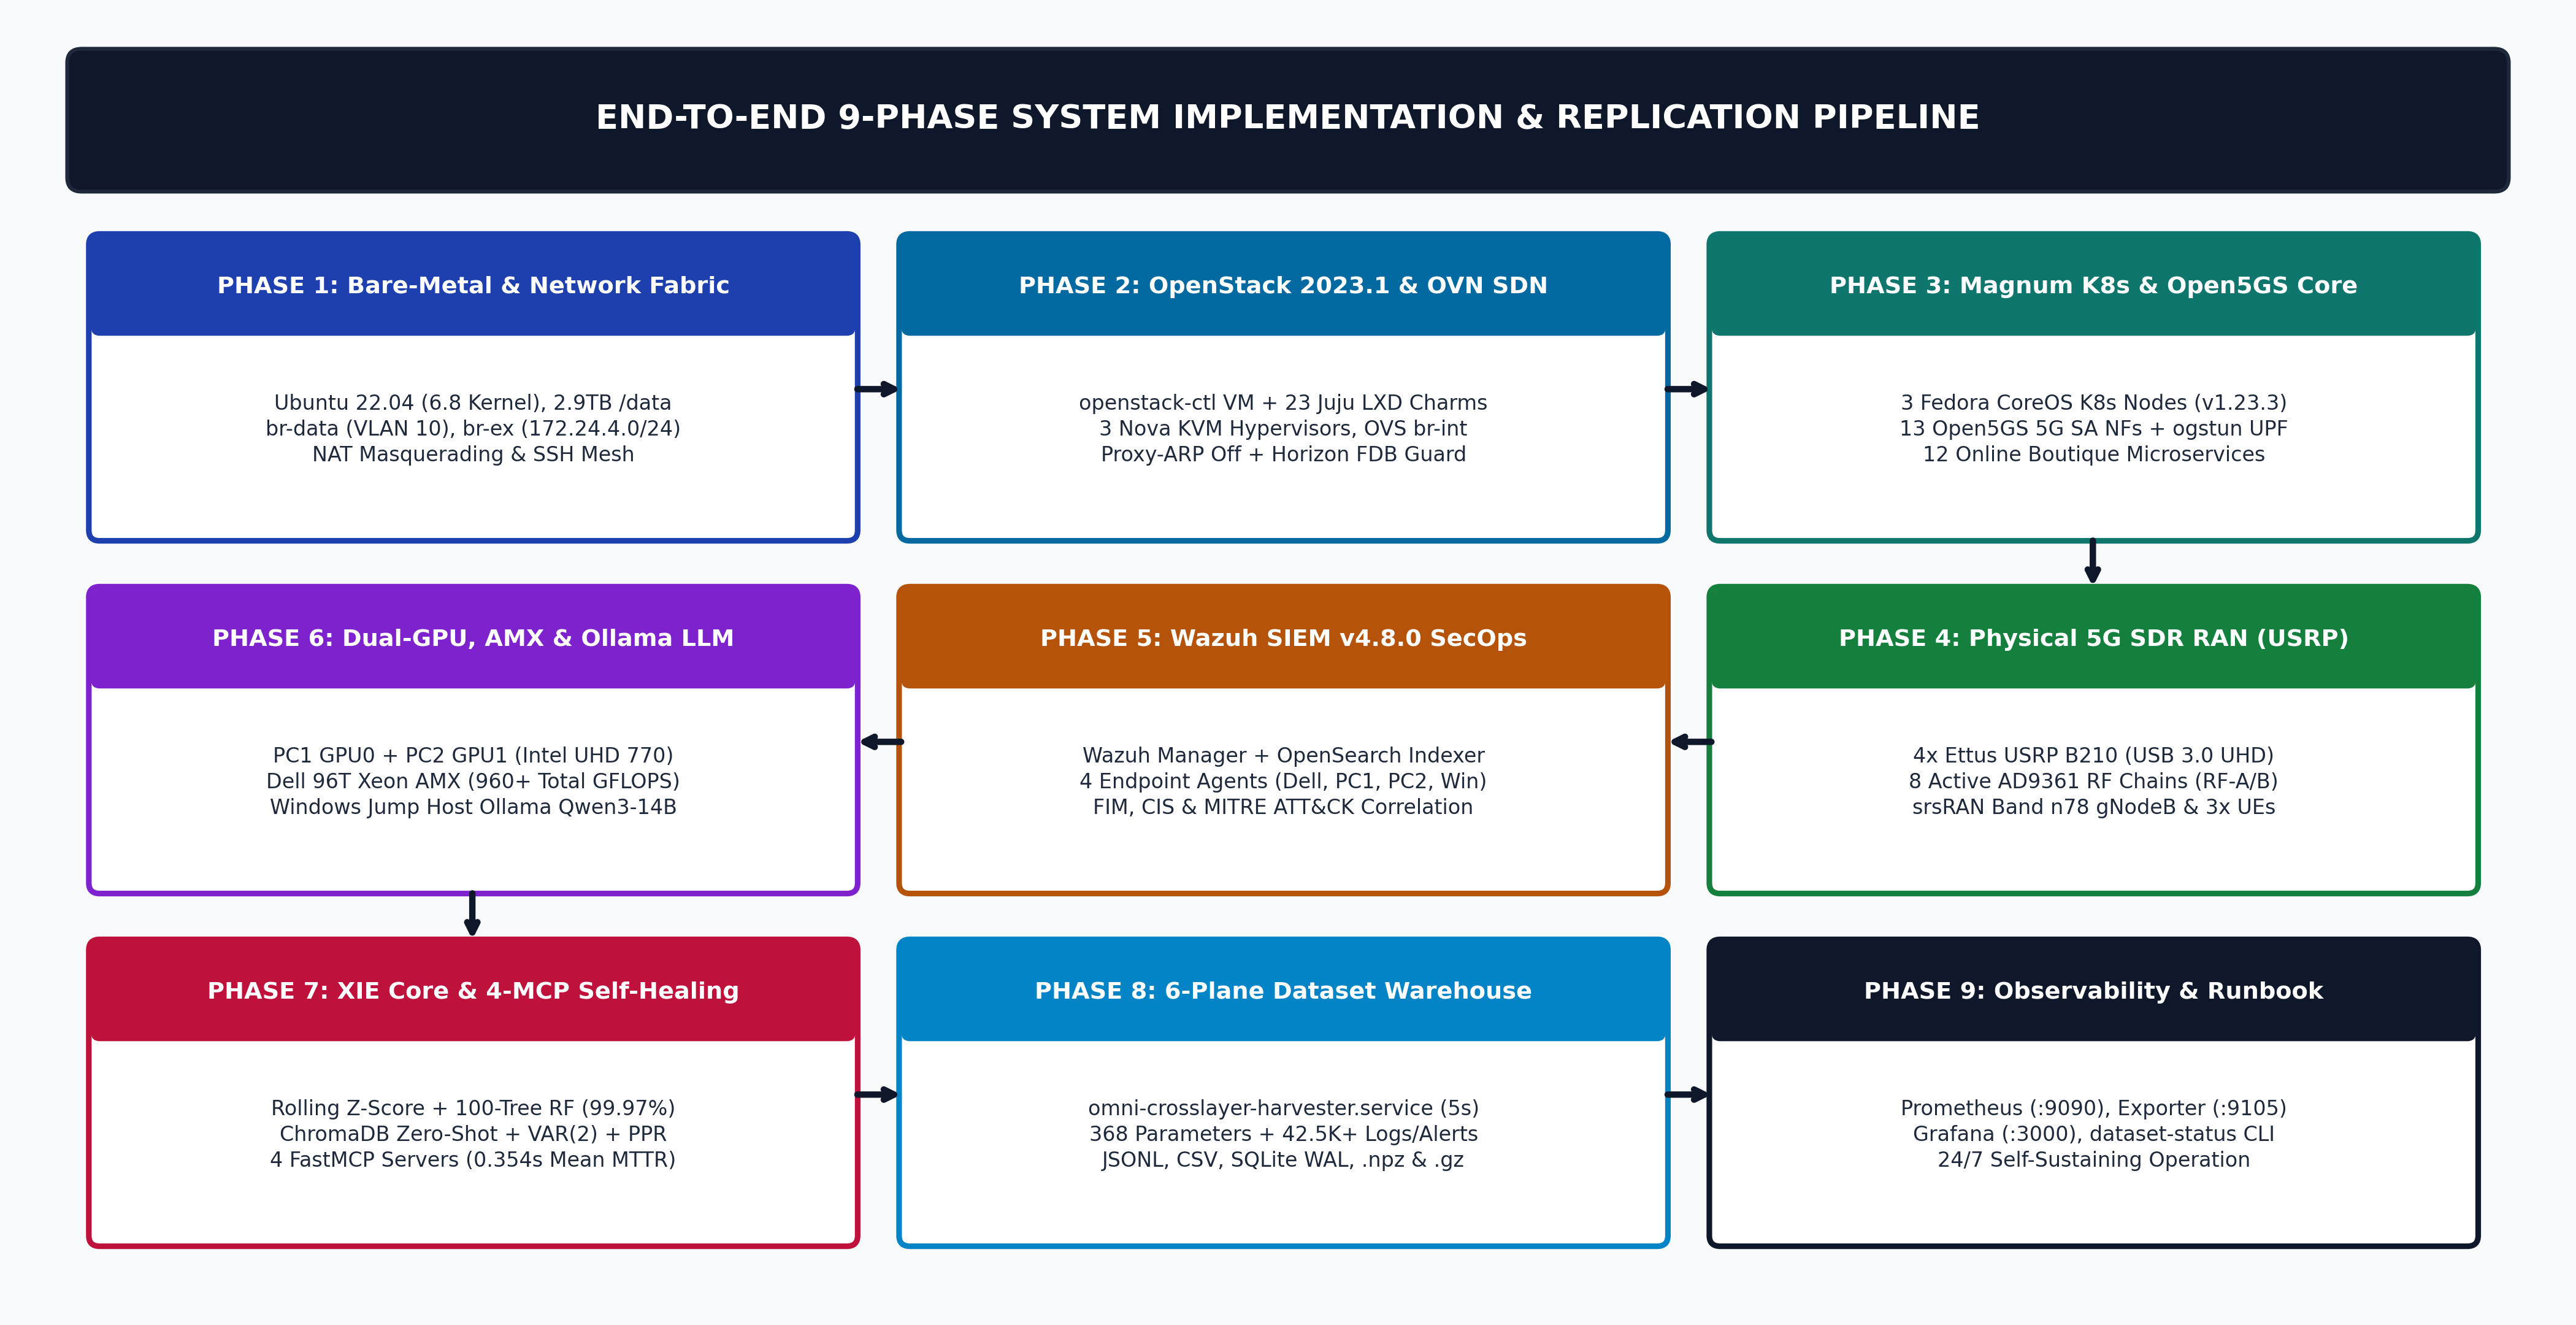
\includegraphics[width=0.98\textwidth]{figures/fig_step_by_step_replication_pipeline.png}
    \caption{End-to-End 9-Phase System Implementation and Replication Pipeline.}
\end{figure}

\subsection{Phase 1: Bare-Metal OS, Enterprise Storage \& Network Bridge Setup}
\begin{lstlisting}[language=bash]
# 1. Mount the 2.9 TB Enterprise Data Array (/dev/sda1) at /data
sudo mkdir -p /data
echo "/dev/sda1 /data ext4 defaults 0 2" | sudo tee -a /etc/fstab
sudo mount -a

# 2. Configure veth pair linking Host Router (172.24.4.254/24) to OVS br-ex
sudo ip link add veth-host type veth peer name veth-br
sudo ip addr add 172.24.4.254/24 dev veth-host
sudo ip link set veth-host up && sudo ip link set veth-br up
sudo ovs-vsctl --may-exist add-br br-ex
sudo ovs-vsctl --may-exist add-port br-ex veth-br

# 3. Enable IPv4 Forwarding & NAT Masquerading
sudo sysctl -w net.ipv4.ip_forward=1
sudo iptables -t nat -A POSTROUTING -s 172.24.4.0/24 ! -d 172.24.4.0/24 -j MASQUERADE
sudo iptables -t nat -A POSTROUTING -s 192.168.100.0/24 ! -d 192.168.100.0/24 -j MASQUERADE
\end{lstlisting}

\subsection{Phase 2: OpenStack 2023.1 Antelope Control Plane, KVM \& Horizon Hardening}
\begin{enumerate}
    \item Provision the LXD VM \texttt{openstack-ctl} (\texttt{10.10.10.3}, 16 vCPUs, 64 GiB RAM) and deploy the 23 Juju OpenStack 2023.1 Antelope containers (\texttt{juju-65b4ac-0-lxd-0} through \texttt{lxd-22}: MySQL InnoDB Cluster Primary \texttt{lxd-10} \texttt{10.10.10.6}, Keystone \texttt{lxd-2} \texttt{10.10.10.9}, Horizon \texttt{lxd-3} \texttt{10.10.10.8}, Nova \texttt{lxd-6} \texttt{10.10.10.13}, Neutron \texttt{lxd-8} \texttt{10.10.10.11}, OVN Central \texttt{lxd-11} \texttt{10.10.10.12}, Magnum \texttt{lxd-15} \texttt{10.10.10.10}, etc.).
    \item \textbf{Permanent Horizon \& Proxy-ARP Hardening:} Disable \texttt{proxy\_arp} on \texttt{br-data} so the Dell host never intercepts intra-container ARP requests on \texttt{10.10.10.0/24}, point Horizon to the writable MySQL Primary (\texttt{10.10.10.6}), and install the root cron guard \texttt{/usr/local/bin/openstack-horizon-guard.sh}:
\end{enumerate}
\begin{lstlisting}[language=bash]
sudo sysctl -w net.ipv4.conf.br-data.proxy_arp=0
sudo sysctl -w net.ipv4.conf.all.proxy_arp=0
sudo /usr/local/bin/openstack-horizon-guard.sh
python3 /home/hpe/test_horizon_login.py
\end{lstlisting}

\subsection{Phase 3: Magnum Kubernetes v1.23.3, Open5GS 5G SA Core \& Online Boutique}
\begin{enumerate}
    \item Deploy the 3-node Fedora CoreOS 35 Kubernetes cluster via Magnum (\texttt{master-0} \texttt{192.168.100.72}, \texttt{node-0} \texttt{192.168.100.131}, \texttt{node-1} \texttt{192.168.100.174}) and export \texttt{/home/hpe/k8s-5g/config}.
    \item Deploy all 13 Open5GS 5G SA Core pods in namespace \texttt{open5gs} (\texttt{nrf}, \texttt{scp}, \texttt{amf}, \texttt{smf}, \texttt{upf}, \texttt{ausf}, \texttt{udm}, \texttt{udr}, \texttt{pcf}, \texttt{nssf}, \texttt{bsf}, \texttt{webui}, \texttt{mongodb-0}) with N2 NGAP SCTP (\texttt{:38412}) and N3 GTP-U (\texttt{:2152}) exposed on \texttt{192.168.100.131}.
    \item Deploy all 12 Google Online Boutique microservices in namespace \texttt{microservices}.
\end{enumerate}

\subsection{Phase 4: Physical 5G SDR RAN (4$\times$ Ettus USRP B210 \& srsRAN Band n78)}
\begin{enumerate}
    \item Connect USRP B210 \texttt{serial=34B18C8} to \texttt{compute-pc1} (\texttt{10.10.10.4}) and configure \texttt{srsgnb.service} on Band n78 TDD (ARFCN 658628, 3879.42 MHz, 20 MHz BW, \texttt{tx\_gain=60}, \texttt{rx\_gain=40}, dual-channel RF-A + RF-B enabled).
    \item Connect the 3 USRP B210 units (\texttt{34B18A2}, \texttt{34B1905}, USRP \#3) to \texttt{compute-pc2} (\texttt{10.10.10.5}) and enable \texttt{srsue1.service}, \texttt{srsue2.service}, and \texttt{srsue3.service} inside isolated network namespaces \texttt{ue1}, \texttt{ue2}, \texttt{ue3}.
\end{enumerate}

\subsection{Phase 5 \& Phase 6: Wazuh SIEM v4.8.0 \& Distributed Dual-GPU / Xeon AMX Compute}
\begin{enumerate}
    \item Enable \texttt{wazuh-manager}, \texttt{wazuh-indexer}, and \texttt{wazuh-dashboard} on Dell R760xs and register Agents \texttt{000} (Dell), \texttt{002} (\texttt{compute-pc1}), \texttt{003} (\texttt{compute-pc2}), and \texttt{004} (\texttt{windows-jump-host}).
    \item Start the distributed AI compute engine (\texttt{/home/hpe/gpu\_and\_cpu\_workload.py}) driving 32 Xeon AMX workers on Dell R760xs ($\sim 545$ GFLOPS) + Intel UHD 770 \texttt{GPU0} on \texttt{compute-pc1} ($\sim 204.6$ GFLOPS) + Intel UHD 770 \texttt{GPU1} on \texttt{compute-pc2} ($\sim 204.6$ GFLOPS) = \textbf{960+ GFLOPS total}.
    \item Start Ollama \texttt{qwen3:14b} on \texttt{10.0.0.21:11434} for automated post-mortem synthesis.
\end{enumerate}

\subsection{Phase 7: Experiential Intelligence Engine (XIE Core) \& 4-Domain FastMCP Servers}
\begin{figure}[htbp]
    \centering
    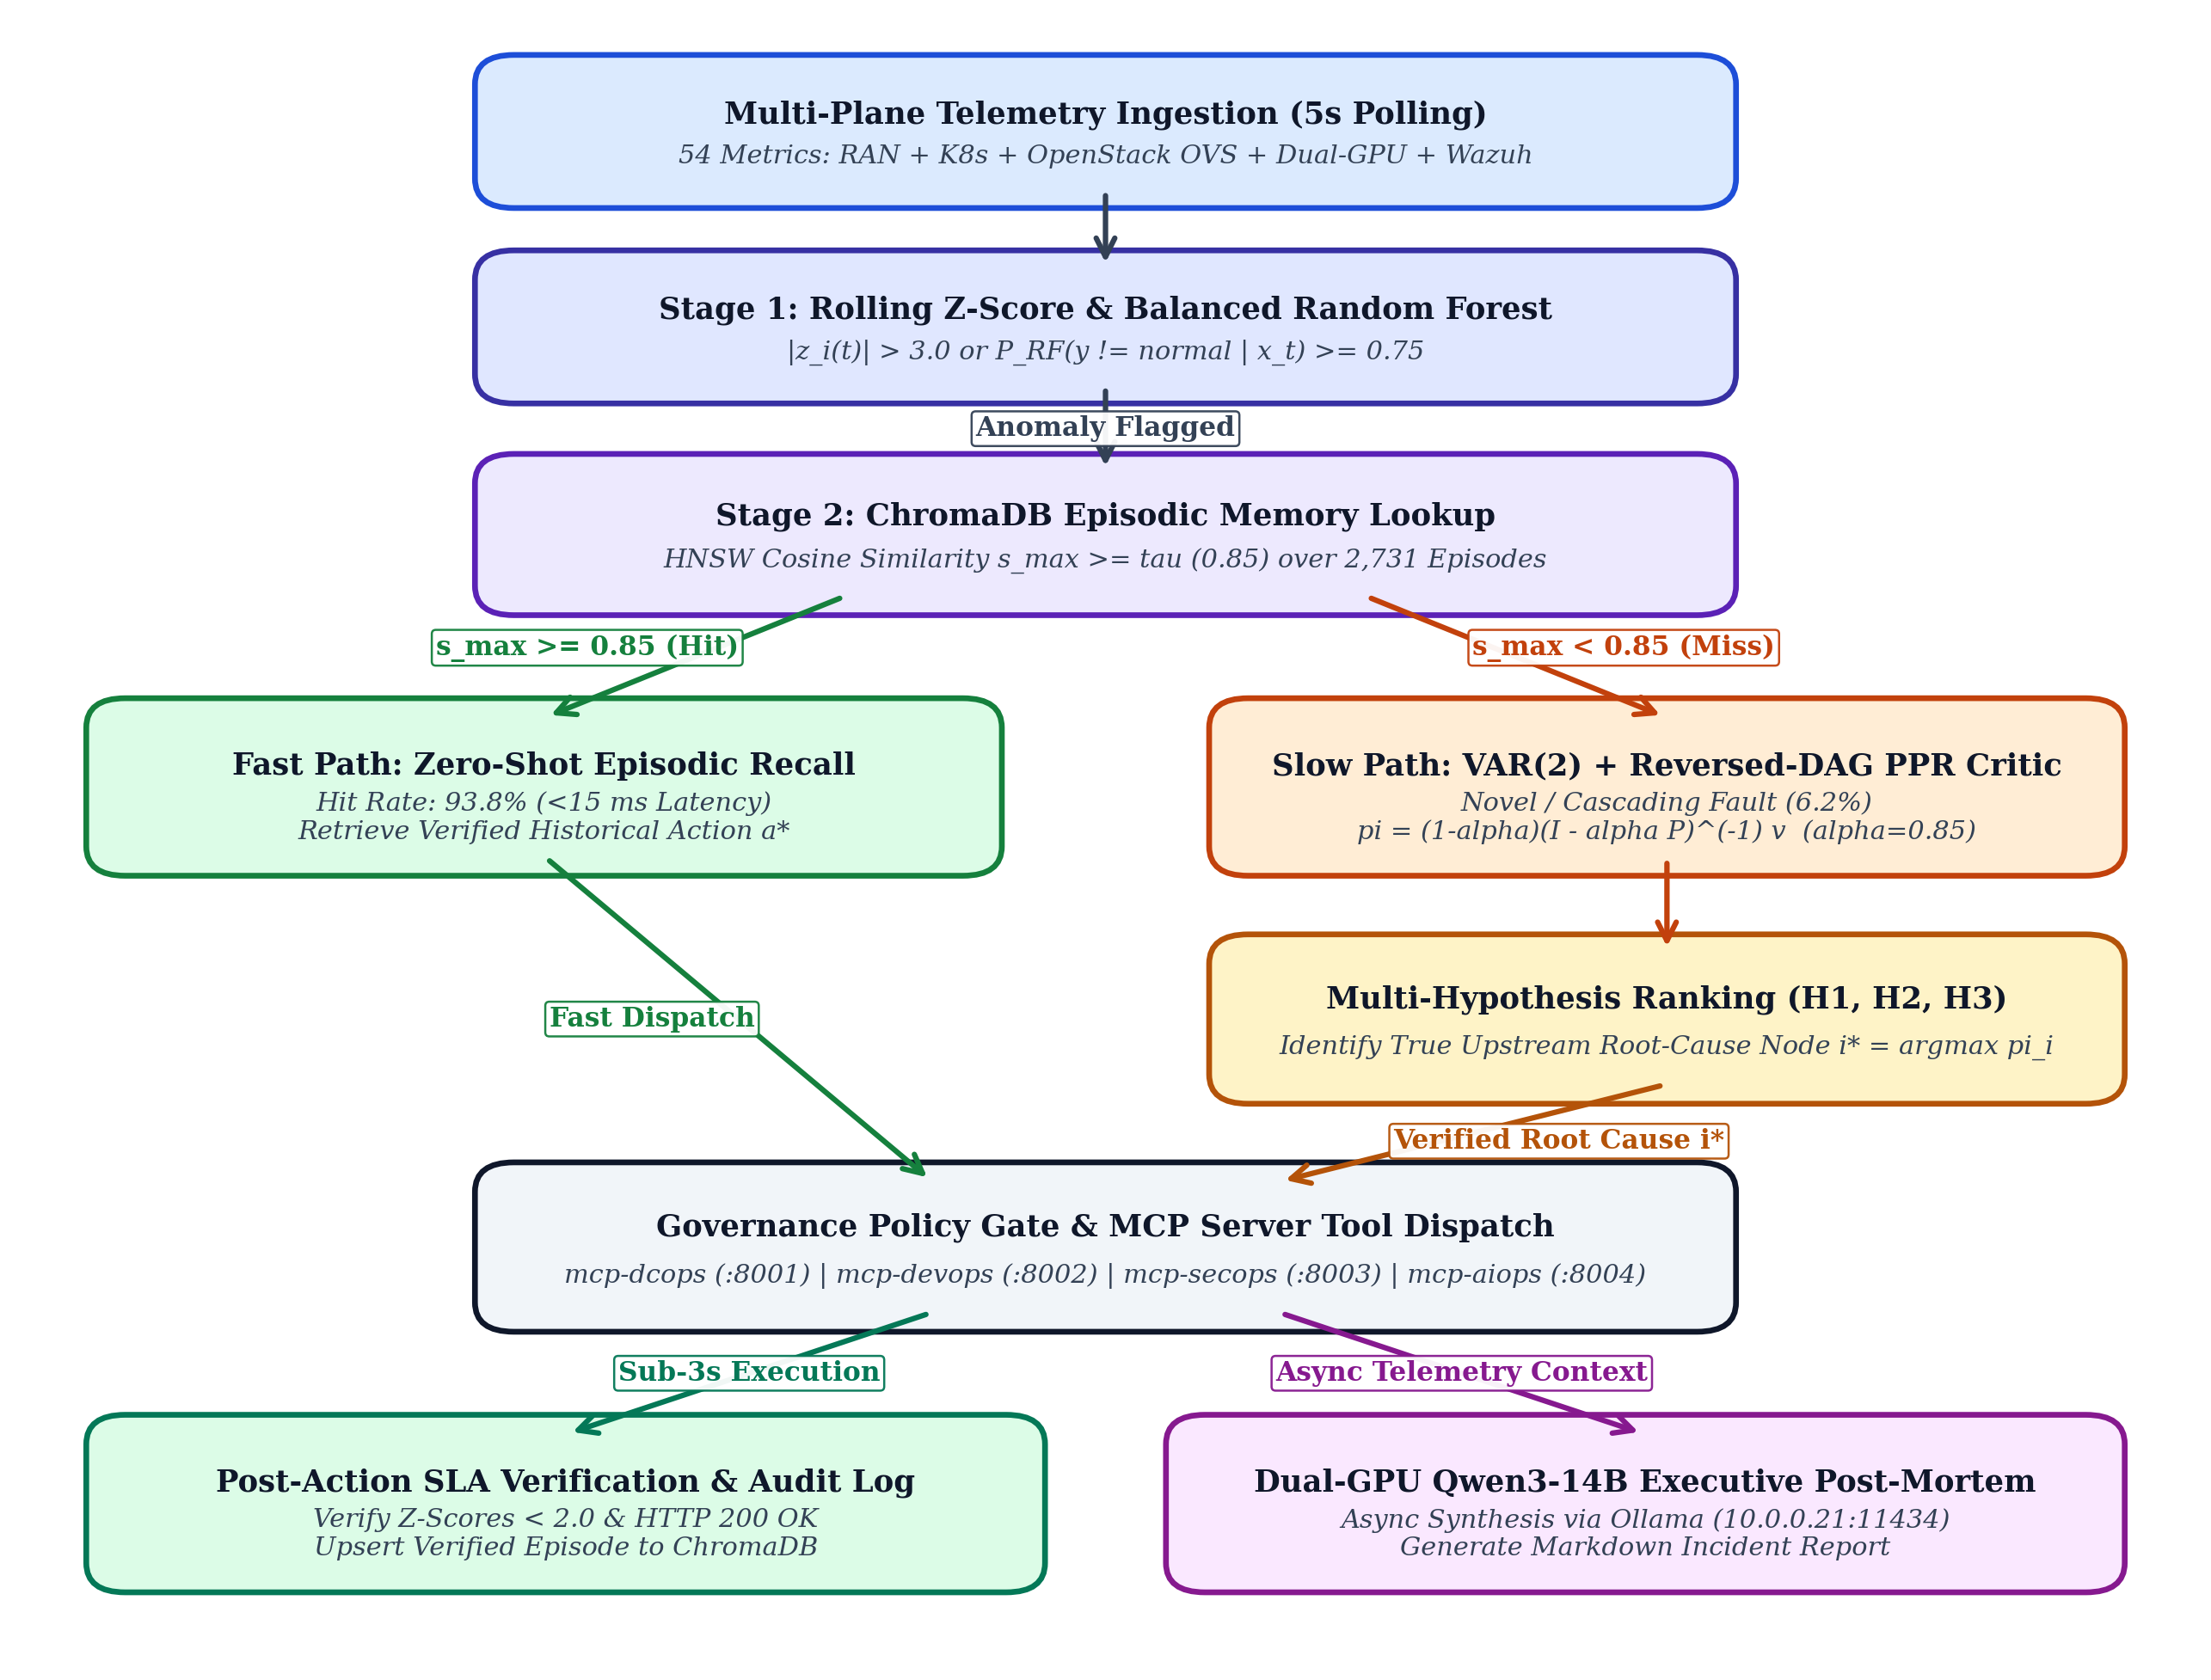
\includegraphics[width=0.82\textwidth]{figures/fig_4_2_agent_flowchart.png}
    \caption{5-Tier Closed-Loop Decision Flowchart of the Experiential Intelligence Engine (XIE Core v1.0).}
\end{figure}
\begin{lstlisting}[language=bash]
# Enable the closed-loop autonomous self-healing agent daemon
sudo systemctl enable --now self-healing-agent.service
tail -n 20 /home/hpe/agent/logs/remediation_audit.log
\end{lstlisting}

\subsection{Phase 8 \& Phase 9: 6-Plane Multi-Dimensional Dataset Warehouse \& Observability}
\begin{figure}[htbp]
    \centering
    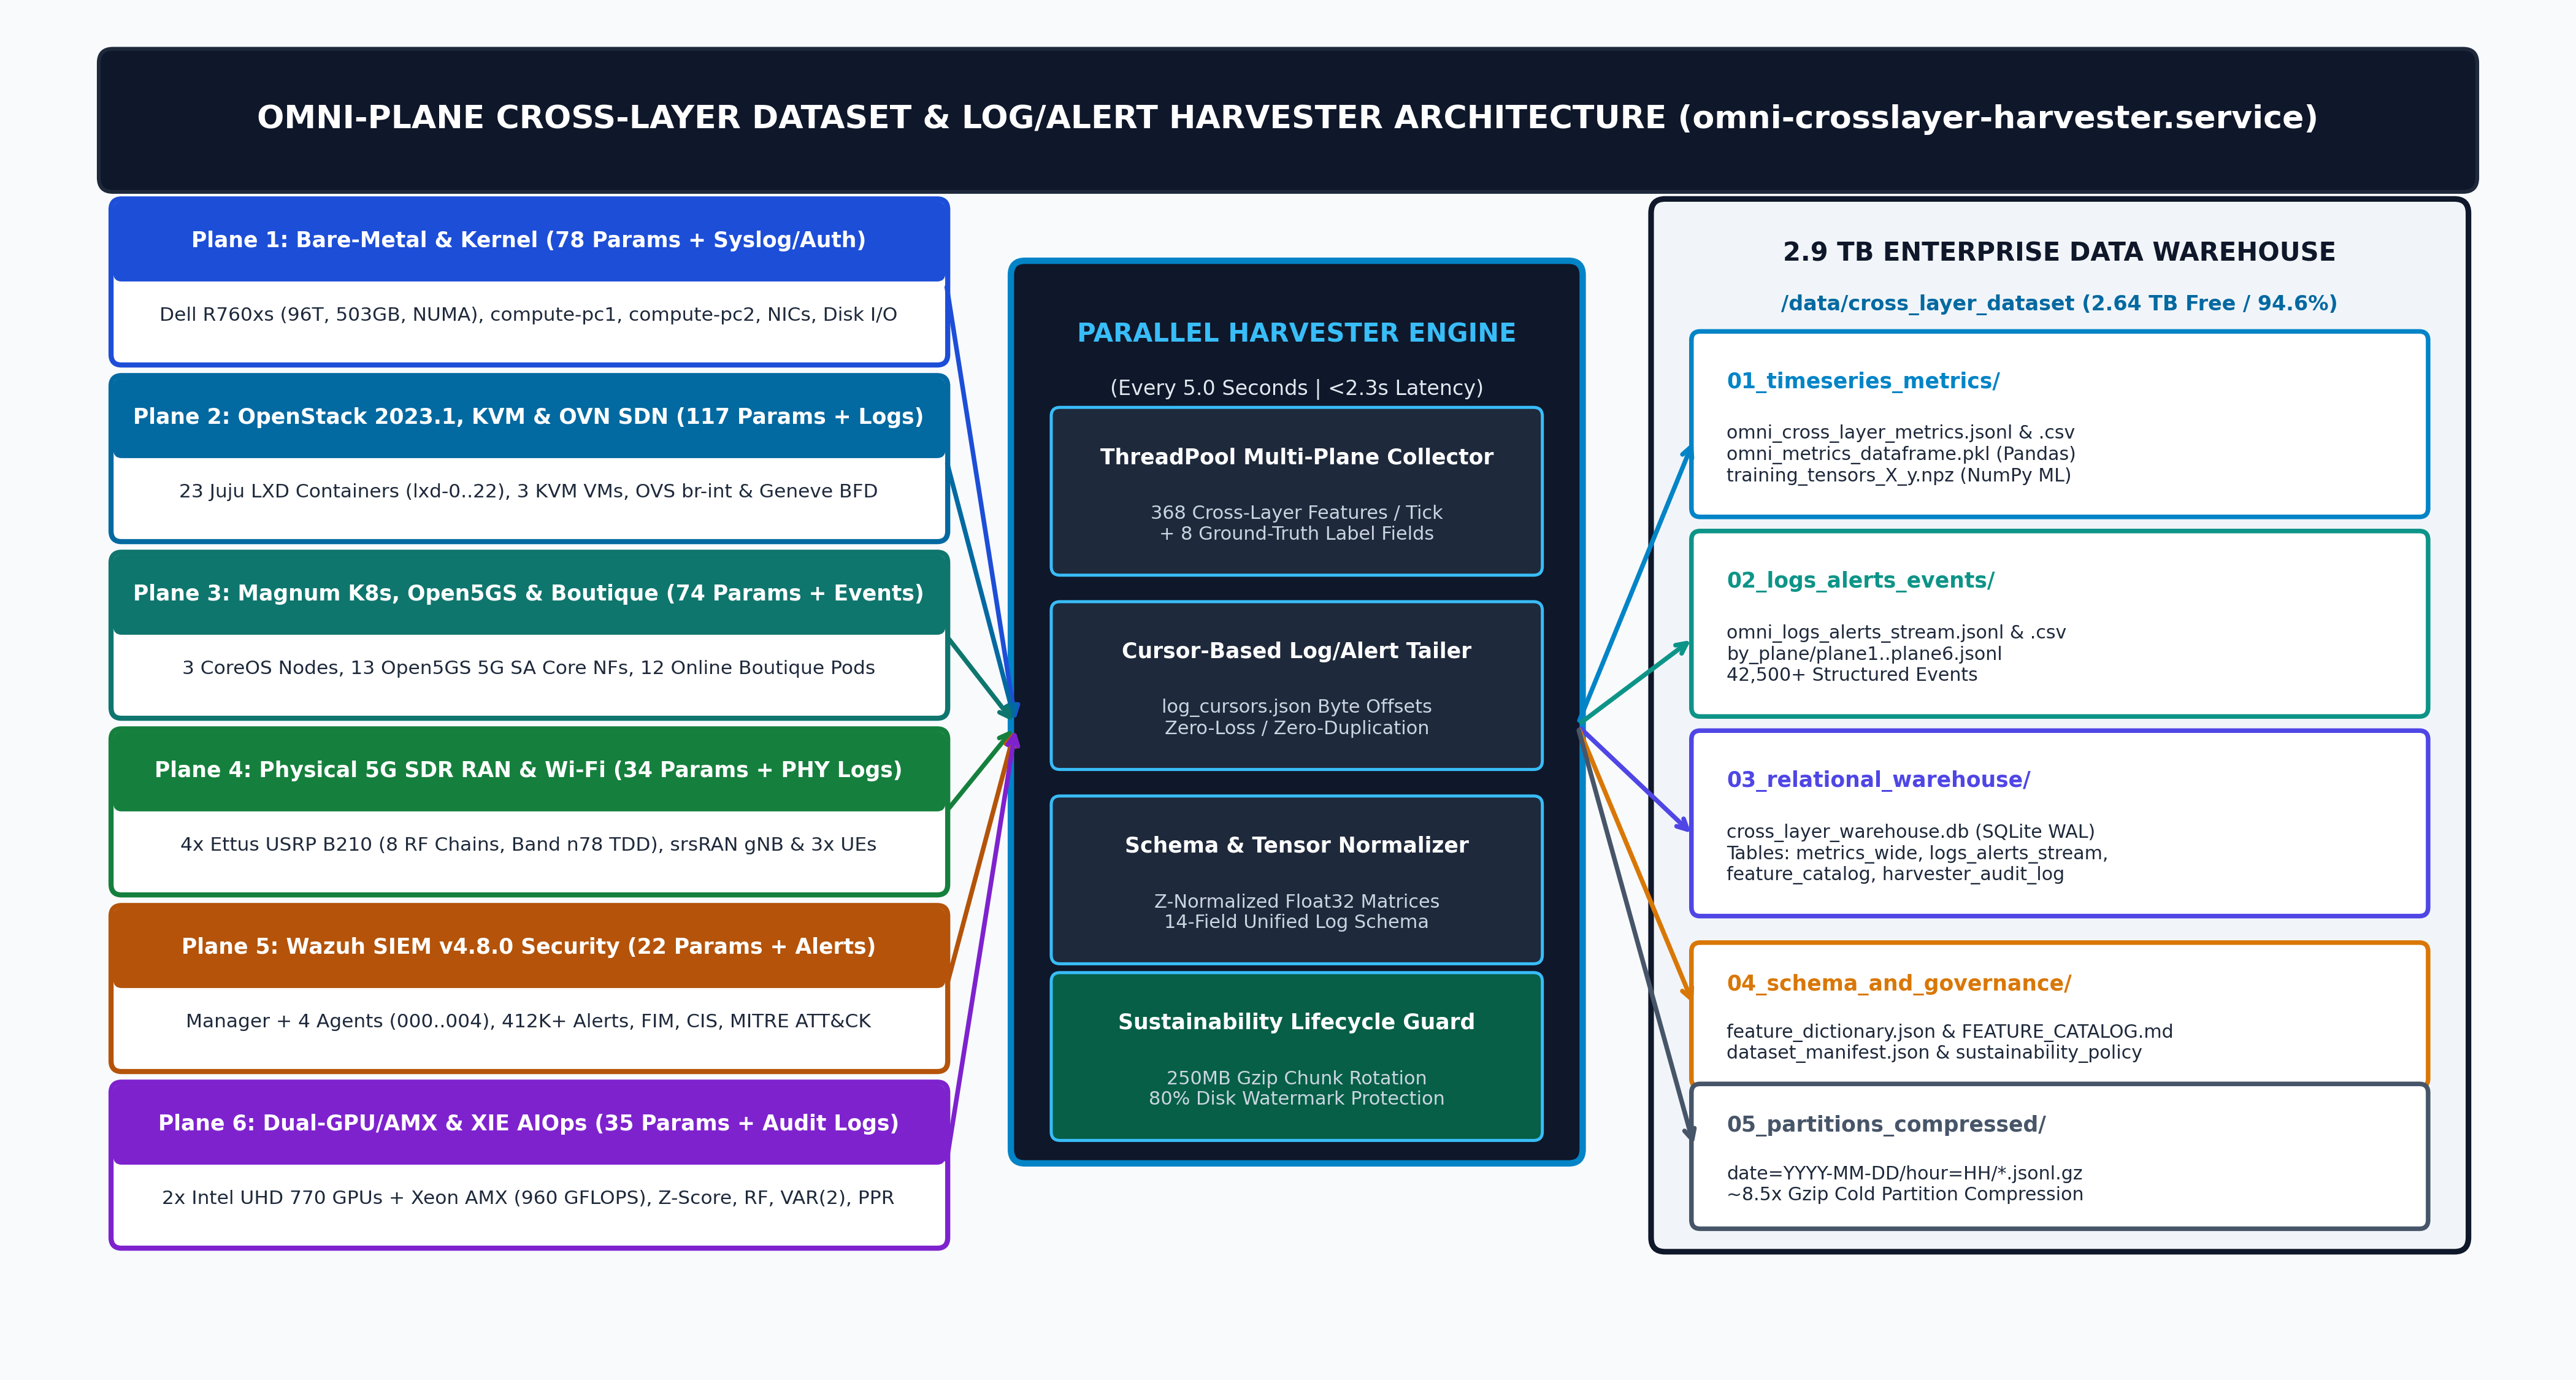
\includegraphics[width=0.98\textwidth]{figures/fig_dataset_warehouse_architecture.png}
    \caption{Architecture of the Continuous 6-Plane Multi-Dimensional Dataset \& Log/Alert Warehouse (\texttt{/data/cross\_layer\_dataset}).}
\end{figure}

The continuous harvester (\texttt{omni-crosslayer-harvester.service}) runs every 5.0 seconds and populates \texttt{/data/cross\_layer\_dataset} (symlinked at \texttt{/home/hpe/HPE/cross\_layer\_dataset}):
\begin{lstlisting}[language=bash]
# Check live dataset warehouse status, row counts, log counts, and latest 368-feature sample
dataset-status

# Check systemd service status
sudo systemctl status omni-crosslayer-harvester.service
\end{lstlisting}

\end{document}

